% ---------------------------------------------------------------
% Preamble
% ---------------------------------------------------------------
%\documentclass[a4paper,fleqn,longmktitle]{cas-sc}
\documentclass[a4paper,fleqn]{cas-dc}
%\documentclass[a4paper]{cas-dc}
%\documentclass[a4paper]{cas-sc}
% ---------------------------------------------------------------
% Make margins bigger to fit annotations. Use 1, 2 and 3. TO be removed later
%\paperwidth=\dimexpr \paperwidth + 6cm\relax
%\oddsidemargin=\dimexpr\oddsidemargin + 3cm\relax
%\evensidemargin=\dimexpr\evensidemargin + 3cm\relax
%\marginparwidth=\dimexpr \marginparwidth + 3cm\relax
% -------------------------------------------------------------------- 
% Packages
% --------------------------------------------------------------------
% Figure packages
\usepackage{graphicx,float}
\usepackage{adjustbox}
% Text, input, formatting, and language-related packages
\usepackage[T1]{fontenc}
\usepackage{subcaption}

\usepackage{csvsimple}

% TODO package
\usepackage[bordercolor=gray!20,backgroundcolor=blue!10,linecolor=black,textsize=footnotesize,textwidth=1in]{todonotes}
\setlength{\marginparwidth}{1in}
% \usepackage[utf8]{inputenc}
% \usepackage[nomath]{lmodern}

% Margin and formatting specifications
%\usepackage[authoryear]{natbib}
\usepackage[sort]{natbib}
\setcitestyle{square,numbers}

 %\bibliographystyle{cas-model2-names}

\usepackage{setspace}
\usepackage{subfiles} % Best loaded last in the preamble

% \usepackage[authoryear,longnamesfirst]{natbib}

% Math packages
\usepackage{amsmath, amsthm, amssymb, amsfonts, bm, nccmath, mathdots, mathtools, bigints, ulem}

\usepackage{tikz}
\usepackage{pgfplots}
\usetikzlibrary{shapes.geometric,angles,quotes,calc}

\usepackage{placeins}

\usepackage[final]{pdfpages}

% --------------------------------------------------------------------
% Packages Configurations
\usepackage{enumitem}
% --------------------------------------------------------------------
% (General) General configurations and fixes
\AtBeginDocument{\setlength{\FullWidth}{\textwidth}}	% Solves els-cas caption positioning issue
\setlength{\parindent}{20pt}
%\doublespacing
% --------------------------------------------------------------------
% Other Definitions
% --------------------------------------------------------------------
\graphicspath{{Figures/}}
% --------------------------------------------------------------------
% Environments
% --------------------------------------------------------------------
% ...

% --------------------------------------------------------------------
% Commands
% --------------------------------------------------------------------

% ==============================================================
% ========================== DOCUMENT ==========================
% ==============================================================
\begin{document} 
%  --------------------------------------------------------------------

% ===================================================
% METADATA
% ===================================================
\title[mode=title]{Optimal design of experiment}                      
\shorttitle{Optimal design of experiment}

\shortauthors{OS, PO}

\author[1]{Oliwer Sliczniuk}[orcid=0000-0003-2593-5956]
\ead{oliwer.sliczniuk@aalto.fi}
\cormark[1]
\credit{a}

\author[1]{Pekka Oinas}[orcid=0000-0002-0183-5558]
\credit{b}

%\author[1]{Francesco Corona}[orcid=0000-0002-3615-1359]
%\credit{c}

\address[1]{Aalto University, School of Chemical Engineering, Espoo, 02150, Finland}
%\address[2]{2}

\cortext[cor1]{Corresponding author}

% ===================================================
% ABSTRACT
% ===================================================
\begin{abstract}
This study aimed to investigate the supercritical extraction process of caraway oil from caraway seeds. The extraction was performed in a partially filled extractor with a fixed bed operated under multiple operating conditions. A distributed-parameter model describes the fluid-solid extraction process with $CO_2$ as a solvent. The concept of quasi-one-dimensional flow is applied to reduce the number of spatial dimensions. The flow is assumed to be uniform across any cross-section, although the area available for the fluid phase can vary along the extractor. 
The optimal design of experiment problem is solved to find an experimental strategy for validating the correlations between extraction kinetic parameters and the operating conditions. This work proposes two experimental strategies: one that only manipulates the inlet temperature and the second that manipulate only the pressure.

\end{abstract}

\begin{keywords}
Supercritical extraction \sep Optimal design of experiment \sep Mathematical modelling \sep Optimization \sep Fisher information
\end{keywords}

% ===================================================
% TITLE
% ===================================================
\maketitle

% ===================================================
% Section: Introduction
% ===================================================\section{Introduction}

\section{Introduction}
%\subfile{Sections/introduction}
\subfile{Sections/introduction_imp}

\subfile{Sections/Literature_Review}

The study is structured as follows: Chapter \ref{CH: Thermodynamic} provides a general discussion on supercritical fluids to familiarize the reader with their properties. Chapter \ref{CH:Governing_equations_chapter} introduces the general balance equations. The balance equations are combined with the extraction kinetic equation to develop the process model in Chapter \ref{CH: Extraction_model}. The derivative-based local sensitivity analysis is presented in Chapter \ref{CH: Sensitivity_Analysis} and is then combined with the process model. Finally, the sensitivity plots are discussed in Chapters \ref{CH: Results} and \ref{CH: Conclusion}.

\section{Materials and methods} \label{CH: Materials and methods}

\subsection{Supercritical fluids} \label{CH: Thermodynamic}
%\subfile{Sections/Thermo}
\subfile{Sections/Thermo_imp}

%\clearpage
%\subfile{Sections/Materials_and_methods}

\subsection{Governing equations} \label{CH:Governing_equations_chapter}
\subfile{Sections/Gouverning_equation}

\subsection{Extraction model} \label{CH: Extraction_model}
\subfile{Sections/Model}

%\newpage
%\section{Bayes theorem} \label{CH: Bayes}
%\subfile{Sections/Bayes_Theorem}
%\clearpage

\subsection{Design of experiment} \label{CH: Optimal_design_of_experiment}
\subfile{Sections/Optimal_design_of_experiment}

%\subsection{Experimental work}
%\subfile{Sections/Experiments}

\section{Results}
%\subfile{Sections/Results_Sensitivity}

\section{Conclusions} \label{CH: Conclusion}



% ===================================================
% Bibliography
% ===================================================
%% Loading bibliography style file
\clearpage
%\bibliographystyle{model1-num-names}
\bibliographystyle{unsrtnat}
\bibliography{mybibfile}

%\clearpage \appendix \label{appendix}
%\section{Appendix} 
%\subsection{Thermodynamic}
%\subfile{Sections/Qubic_EOS}

%\subsection{Governing equations}
%\subfile{Sections/Gouverning_equation_derivation}

%\subsection{Low Mach number expansion} \label{CH:Low_Mach_chapter}
%\subfile{Sections/Low_mach_number_expansion}
%\subfile{Sections/Low_mach_number_expansion_imp}

%\subsection{Bayes theorem} \label{CH: Bayes}
%\subfile{Sections/Bayes_Theorem}

%\subsection{Cardano's Formula} \label{CH: Cardano}
%\subfile{Sections/Cardano}

%\subsection{Initial and boundary conditions} \label{CH: IC_BC}
%\subfile{Sections/IC_BC}

%\subsection{Maximum Likelihood} \label{CH: ML}
%\subfile{Sections/Likelihood}

%\subsection{Solid density measurement} \label{CH: Solid_Density_Measurment}

%\begin{figure}[!h]
%	\centering 
%	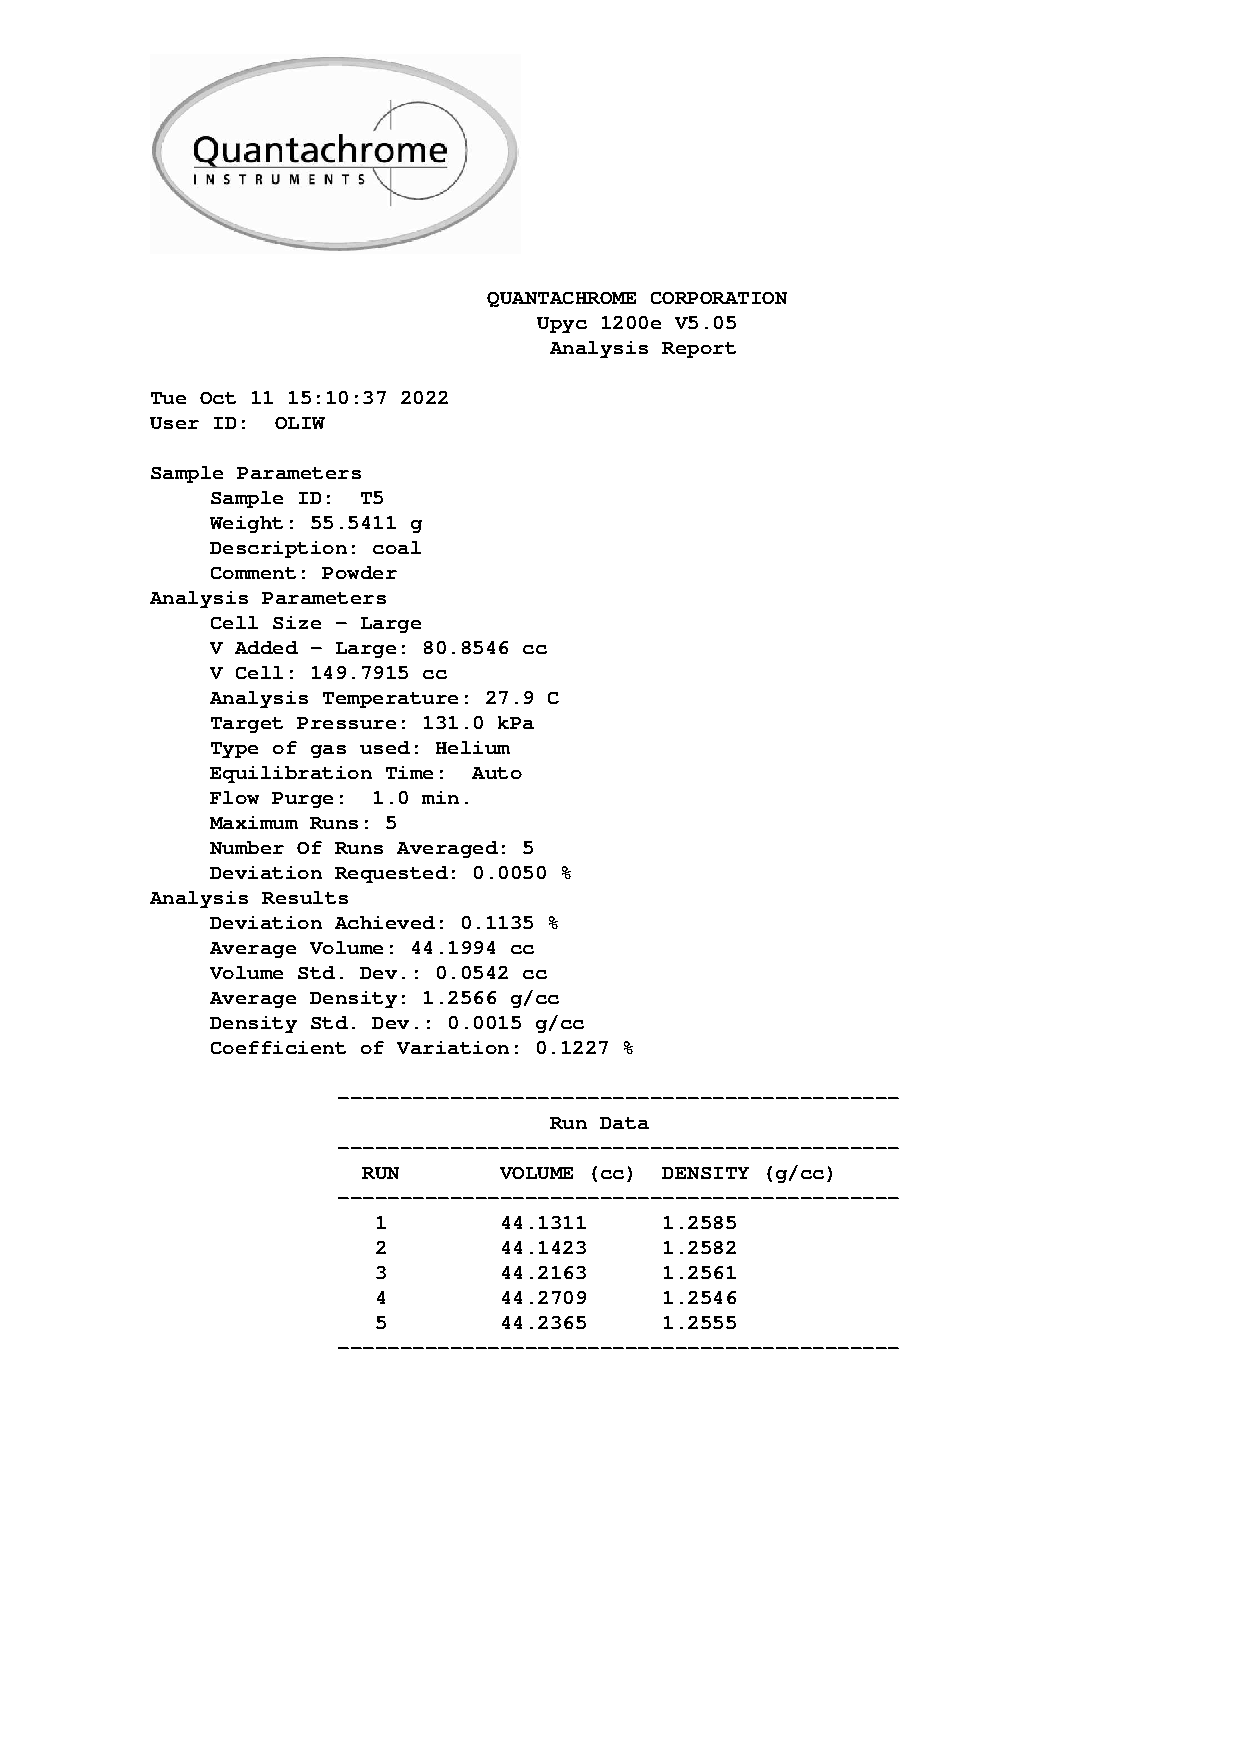
\includegraphics[trim=2cm 6cm 4cm 0cm, clip,width=\columnwidth]{Sections/ultraReportT5.pdf}
%	\caption{The result of solid density measurement}
%\end{figure}

%{\footnotesize
%	\begin{equation*}
%		\rho_s^{ave} = \frac{1.2585+1.2582+1.2561+1.2546+1.2555}{5} = 1.25658 [g/cc]
%	\end{equation*} }

%\subsection{Porosity Calculations} \label{CH: Porosity}
%\subfile{Sections/Porosity}

%\subsection{Concentration profiles} \label{CH: Profiles}
%\subfile{Sections/Profiles}

%\subsection{Solution of the parameter estimation starting from another initial guess} \label{CH: Profiles_2}
%\subfile{Sections/Parameter_estimation_solution_from_another_IG}

\end{document}